\chapter{Results}
This chapter contains the results of the thesis. First, we look at the outcomes of the user test.
The results are encouraging and we take a closer look at some of them.
Then, small applications demonstrate the usage of the Sequence Library. The
examples show that the concepts and implementations presented in this thesis
are useful in different ways. The following section lists features that have not yet been
implemented. Finally, we will discuss the results obtained in this thesis. For
this purpose, we will take a closer look at the specific topics of this work.
Each topic briefly mentions what was achieved and where there were limits to
it.
\section{User Test Evaluation} % (fold)
\label{sec:User Test Evaluation}
\subsection{Introduction} % (fold)
\label{sub:Introduction}
We conducted user tests with various developers to get feedback on the library.
In total, 13 people participated in this test. All those received a link to a
GitHub repository containing the description of two tasks:
\begin{enumerate}
\item \textbf{Numerical differentiation}: The idea is to use sequences to get
  an approximation as close as possible to the slope of a function |f| at point
  |x|. Lazyness and operations on sequences make this possible.
\item \textbf{Browse JSON files}: In JavaScript you frequently work with JSON
  files provided by some API. This data is often full of holes, which makes it
  difficult to process. JINQ simplifies this task significantly because it
  fills such gaps automatically. 
\end{enumerate}
Both tasks are pleasent use cases of the artifacts of this work.
Chapter~\ref{sec:Examples} describes them in detail.\\
Finally, each participant filled out a questionnaire. This procedure enables
the detection of difficulties and shows where the API still has room for
improvement. 

The findings are based on the questionnaire evaluation and the code of three
participants who handed in their solution. This chapter lists all the
improvements the user test pointed out. In addition, it concludes the general
impression collected by the user test.
Appendix~\ref{chap:app_user_test_results} contains all the user test questions
and their answers.
% subsection Introduction (end)
\subsection{Findings for the Sequence library} % (fold)
\label{sub:Findings for the sequence library}
\subsubsection{Findings and Improvements} % (fold)
\label{subsub:seq_findings_and_improvements}
We decided to include following findings in the Sequence library:
\begin{itemize}
  \item \textbf{Renaming untilFunction}: Creating sequences using the sequence
    constructor worked well for everyone. The meaning of the parameters was
    clear to all (\ref{sub:ut_q3}). However, a suggestion for a meaningful
    optimization from two participants was to rename the |untilFunction| to
    |whileFunction|. This name states clearer that the function should return
    |false| when the sequence ends. (This suggestion was handed in by a
    solution)
  \item \textbf{Better type documentation in JSDoc}: The IDEs have problems
    correctly displaying type information for curried functions (Ref. 2).
    Therefore, the already often used JSDoc annotation |@haskell| , which
    describes the type signature of a function as in Haskell, is added
    everywhere.
\end{itemize}
The following are great ideas but are beyond the scope of this project to
implement. Find detailed information about all of them in the
Section~\ref{sub:Operators and Operations}.
\begin{itemize}
  \item \textbf{unfoldr}: This suggestion was handed in by a solution
  \item \textbf{uncons with empty sequences}: This suggestion was handed in by a solution
\end{itemize}

\subsubsection{Conclusion} % (fold)

Almost everyone uses operators as |map|, |filter|, |take|, |reduce|
frequently when working with lists. So the Sequence library brings much-needed
functions. (\ref{sub:ut_q2}) \\ 
Figure~\ref{fig:usertest_q1} concludes the overall opinion about the Sequence
library very well. It shows that most users think that it can be an
advantage in their next project.
\begin{figure}[H]
  \centering
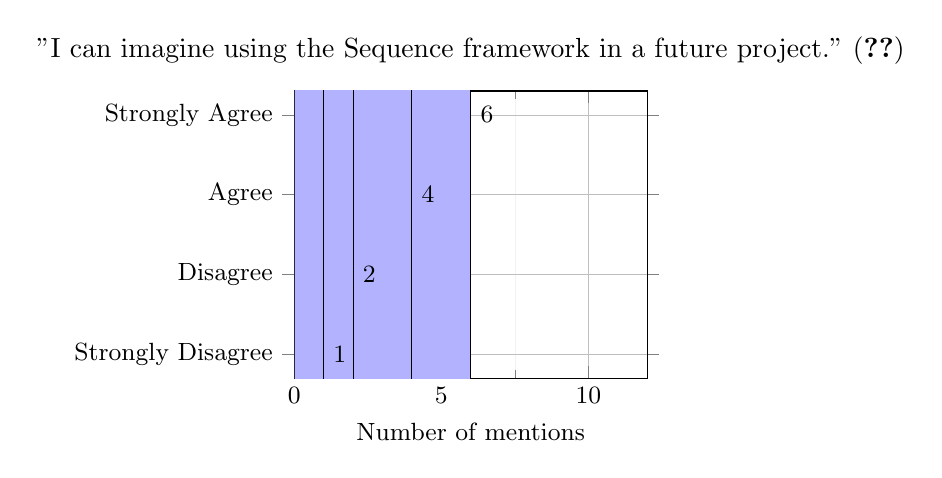
\begin{tikzpicture}
\begin{axis}[
% instead of scaling
width=\textwidth / 2, % Breite des Charts
title={"I can imagine using the Sequence framework in a future project."~(\ref{sub:ut_q4})},
xbar,  % Art des Charts                                            
xmin=0, % y min
xmax=12, % y max
%ylabel style={color=darkgray},
ticklabel style={font=\small},
label style={font=\small},
nodes near coords style={font=\small},
bar width=20, % Breite der Balken (in points)
nodes near coords, % Labels oberhalb der Bars
xlabel={Number of mentions},
grid=both, % Zeilen ds Grids
grid style={line width=.1pt, draw=gray!10},
major grid style={line width=.2pt,draw=gray!50},
minor x tick num=1,
ytick=data,
% use explicit ticklabels instead of symbolc x coords
yticklabels={Strongly Agree, Agree, Disagree, Strongly Disagree},
]
\addplot[black,fill=blue!30!white]
coordinates{ (6,4) (4,3) (2,2) (1,1) };
\end{axis}
\end{tikzpicture}
\caption{Responses to "I can imagine using the Sequence framework in a future project."}
\label{fig:usertest_q1}
\end{figure}
% subsubsection Conclusion (end)
% subsection Findings Sequence library(end)
\subsection{Findings for JINQ} % (fold)
\label{sub:Findings for JINQ}
\subsubsection{Findings and Improvements} % (fold)
\label{subsub:jinq_finding_and_imrpovements}

We decided to include following findings into JINQ:
\begin{itemize}
  \item \textbf{Better Introduction to JINQ}: Two people suggest using
    |JSONMonad()| directly inside of |from| (text answer~\ref{sub:ut_q13}).
    However, this makes no sense since JINQ can handle arbitrary monads. Thus,
    the documentation provided did not provide a sufficient overview.
    Therefore, the JSDoc of JINQ must give a better introduction to the topic.
    Additional examples should show the usage using different monads.
  \item \textbf{Revise JSDoc (functions and examples)}: Nearly a quarter of the participants found JINQ
    challenging (\ref{sub:ut_q8}). This shows that these concepts needed to be
    sufficiently well introduced. From the solutions given to us, it is evident
    that more JSDoc was required. In addition, more examples would coin to a
    better understanding (text answer~\ref{sub:ut_q13}).
    \item \textbf{Not exactly the same as SQL}: Two people needed help with
      JINQ not writing exactly like SQL (handed in code). An SQL query
      |Select NAME from PERSON where AGE > 18| is translated into JINQ via
      |from(PERSON).where(p => p.age > 18).select(p => p.name);| So the order
      of |select| and |where| is reversed. So the JSDoc of JINQ needs to
      mention more clearly that working with JINQ is different than working
      with SQL.
\end{itemize}

The following are great ideas but are beyond the scope of this project to
implement. Find detailed information about all of them in the
Section~\ref{sub:JINQ Functions}.
\begin{itemize}
  \item \textbf{Error handling}: Several people had trouble with null values,
    mainly when, for example, when calling a  function on a non-existent object
    property in a |select| or a |where| (text answer~\ref{sub:ut_q13}, and
    handed in solution). In the discussion, the idea came up to
    provide functions like |notNull|, |safeWhere| or |safeMap| to catch this.
\end{itemize}
% subsubsection Findings and Improvements (end)
\subsubsection{Conclusion} % (fold)
\label{subsub:Conclusion}
Although JINQ still has room for improvement, the general feedback is very
good. Almost all find it helpful to search JSON structures using JINQ
(\ref{sub:ut_q10}). The majority already found the current state of JINQ easy
to use \ref{sub:ut_q8}.

As Figure~\ref{fig:usertest_q2} shows, most people think that JINQ can be an asset in a future
project:
\begin{figure}[H]
\centering
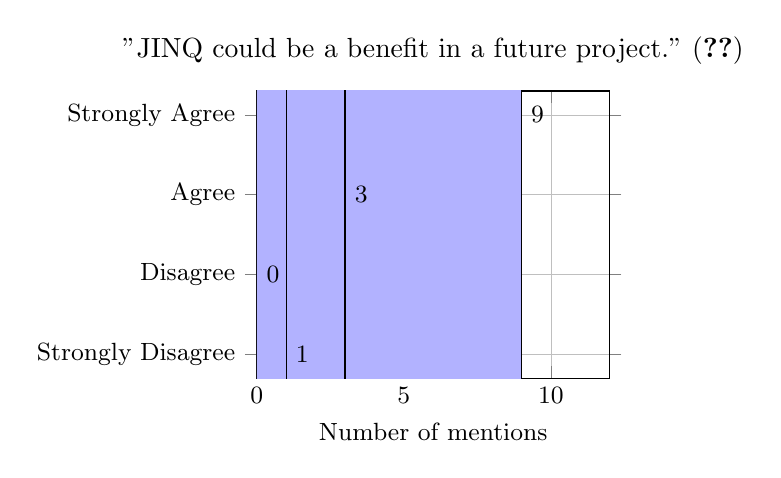
\begin{tikzpicture}
\begin{axis}[
% instead of scaling
width=\textwidth / 2, % Breite des Charts
title={"JINQ could be a benefit in a future project."~(\ref{sub:ut_q12})},
xbar,  % Art des Charts                                            
xmin=0, % y min
xmax=12, % y max
%ylabel style={color=darkgray},
ticklabel style={font=\small},
label style={font=\small},
nodes near coords style={font=\small},
bar width=20, % Breite der Balken (in points)
nodes near coords, % Labels oberhalb der Bars
xlabel={Number of mentions},
grid=both, % Zeilen ds Grids
grid style={line width=.1pt, draw=gray!10},
major grid style={line width=.2pt,draw=gray!50},
minor x tick num=1,
ytick=data,
% use explicit ticklabels instead of symbolc x coords
yticklabels={Strongly Agree, Agree, Disagree, Strongly Disagree},
]
\addplot[black,fill=blue!30!white]
coordinates{(9,4) (3,3) (0,2) (1,1)};
\end{axis}
\end{tikzpicture}
\caption{Responses to "JINQ could be a benefit in a future project."}
\label{fig:usertest_q2}
\end{figure}
% subsubsection Conclusion (end)
% subsection Findings for JINQ (end)
\subsection{General Findings} % (fold)
\label{sub:General Findings}
The questionnaire concludes with general questions. Among other things, the
closing explains how effectively IDEs support JSDoc and whether the testers
find this useful. Most participants used IntelliJ or WebStorm for testing
(~\ref{sub:ut_q15}). Figure~\ref{fig:usertest_q3} shows that the IDE was an excellent help for this test. Thus, It
makes sense to write a detailed JSDoc. Code navigation, code completion, etc.,
are also popular with users in JavaScript. With the right IDEs, this also works
very well.
%\begin{figure}[H]
%\begin{tikzpicture}
%\begin{axis}[
%% instead of scaling
%width=\textwidth / 2, % Breite des Charts
%title={"My IDE provided me with helpful support during the user test." (\ref{sub:ut_q16})},
%ybar,  % Art des Charts                                            
%ymin=0, % y min
%ymax=12, % y max
%%ylabel style={color=darkgray},
%%xlabel style={font=\small},
%bar width=20, % Breite der Balken (in points)
%nodes near coords, % Labels oberhalb der Bars
%ylabel={Number of mentions},
%grid=both, % Zeilen ds Grids
%grid style={line width=.1pt, draw=gray!10},
%major grid style={line width=.2pt,draw=gray!50},
%minor y tick num=4,
%xtick=data,
%% use explicit ticklabels instead of symbolc x coords
%xticklabels={Strongly Agree, Agree, Disagree, Strongly Disagree},
%xticklabel style={ rotate=-20 },
%]
%\addplot[black,fill=blue!30!white]
%coordinates{ (1,10) (2,2) (3,1) (4,0) };
%\end{axis}
%\end{tikzpicture}

\begin{figure}[H]
\centering
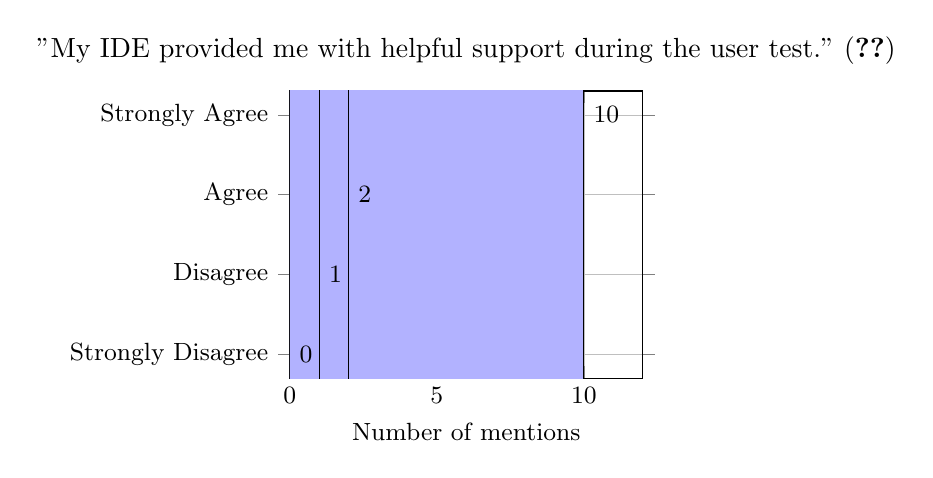
\begin{tikzpicture}
\begin{axis}[
% instead of scaling
width=\textwidth / 2, % Breite des Charts
title={"My IDE provided me with helpful support during the user test." (\ref{sub:ut_q16})},
xbar,  % Art des Charts                                            
xmin=0, % y min
xmax=12, % y max
%ylabel style={color=darkgray},
ticklabel style={font=\small},
label style={font=\small},
nodes near coords style={font=\small},
bar width=20, % Breite der Balken (in points)
nodes near coords, % Labels oberhalb der Bars
xlabel={Number of mentions},
grid=both, % Zeilen ds Grids
grid style={line width=.1pt, draw=gray!10},
major grid style={line width=.2pt,draw=gray!50},
minor x tick num=1,
ytick=data,
% use explicit ticklabels instead of symbolc x coords
yticklabels={Strongly Agree, Agree, Disagree, Strongly Disagree},
]
\addplot[black,fill=blue!30!white]
coordinates{ (10,4) (2,3) (1,2) (0,1) };
\end{axis}
\end{tikzpicture}
\caption{Responses to "My IDE provided me with helpful support during the user
test."}
\label{fig:usertest_q3}
\end{figure}

% subsection General Findings (end)
\subsection{Conclusion} % (fold)
\label{sub:Conclusion}

This user test shows that the features this library brings are beneficial. In
addition, it offers some improvement points of the API. Implementing the
documented hints improves the quality and usability of this library even more.
We are delighted with the result. Of course, we are especially pleased with the
text responses - many further underline the positive attitude towards this
library. 

% subsection Conclusion (end)
% section User Test Evaluation (end)

\section{Examples} % (fold)
\label{sec:Examples}
This section shows some examples implemented with the
Sequence library to demonstrate its variable usage.
The following covers easy-to-understand and more sophisticated
examples. Consult the listed sources to understand the applications
thoroughly if something is unclear.

\subsection{Fibonacci Sequence}
\label{sub:Fibonacci Sequence}
This is an example of a specialized sequence constructor.
Listing~\ref{lst:fibonacci_sequence} shows the implementation of the Fibonacci 
sequence~\cite[p.~36]{math_diskrete_2011}:
\begin{lstlisting}[
  style=ES6, 
  caption=FibonacciSequence implementation,
  label={lst:fibonacci_sequence}
  ]
const start   = Pair(0)(1);
const whileFn =  _ => true;
const incrFn  = ([fst, snd]) => Pair(snd)(fst + snd);
/**
 * Generates the Fibonacci sequence.
 *
 * @constructor
 * @pure
 * @returns { SequenceType<Number> }
 *
 * @example
 * const result = take(8)(FibonacciSequence);
 *
 * console.log(...result);
 * // => Logs '1, 1, 2, 3, 5, 8, 13, 21'
 */
const FibonacciSequence = 
                    map(pair => pair(snd))(Sequence(start, whileFn, incrFn));
\end{lstlisting}
The |FibonacciSequence| constructor generates the Fibonacci sequence using the
|Sequence| and |Pair| constructors. The incrementation function produces a pair
containing the last returned value and the value to be returned.  The |map|
function then extracts the current Fibonacci number from the pair returned by
the sequence.

\subsection{Fizz Buzz}
\label{sub:Fizz Buzz}
Fizz Buzz is a simple game played with numbers, typically in a group setting. Players
take turns counting upward, but instead of saying numbers divisible by 3, they
say "Fizz", and instead of numbers divisible by 5, they say "Buzz". If a number
is divisible by both 3 and 5, they say "FizzBuzz". This game also serves as a 
programming task.
\newline
Frege Goodness~\cite{frege_goodness} includes a detailed explanation of the
game. 

First, let us look at the game's simplest form in listing~\ref{lst:simple_fizzbuzz}. 
The fizzes and buzzes are combined in a sequence. 
The sequence returns a number if neither a fizz nor a buzz occurs:

\begin{lstlisting}[
  style=ES6, 
  caption=Fizz Buzz example,
  label={lst:simple_fizzbuzz}
  ]
const limit    = 15;
const range    = Range(1, limit);
const fizzez   = cycle(["", "", "fizz"]);
const buzzez   = cycle(["", "", "", "", "buzz"]);

const pattern  = zipWith((fizz, buzz) => fizz + buzz)(fizzez)(buzzez);
const fizzbuzz = zipWith((num, str) => str === "" ? num : str)(range)(pattern);

console.log(...take(limit)(fizzbuzz));
// => Logs '1 2 "fizz" 4 "buzz" ... 11 "fizz" 13 14 "fizzbuzz"'
\end{lstlisting}

As you observe, the entire setup relies on sequences. We define three
distinct endless sequences. A range generates a line of numbers, while |cycle|
produces an unending repetition for "fizzes" and "buzzes". Memory usage remains
minimal. Subsequently, |zipWith| merges the individual sequences and yields a
new sequence. This uncomplicated setup underscores that working with sequences
is declarative, straightforward and highly understandable.

Now we are extending the application to add new rules during the runtime:

\begin{lstlisting}[
  style=ES6, 
  caption=Fizz Buzz example extended,
  label={lst:fizz_buzz}
  ]
import * as _ from "./src/sequence/sequence.js";

const infiniteNumbers = _.Sequence(1, _ => true, i => i + 1);

const createSequenceForRule = rule =>
  _.pipe(
    // add rule's text to number
    _.map(a => a === rule.getNr() ? rule.getText() : ""),     
    _.take(rule.getNr()), // abort on this rules number
    _.cycle
  )(infiniteNumbers);

const buildFizzBuzz = () => {
  const currentRules = model.rulesSnapshot().map(createSequenceForRule);
  const baseLine     = _.Sequence("", _ => true, _ => "");

  const fizzBuzz = _.pipe(
      // reduce to single sequence by combining all iterable values
    _.reduce$((acc, cur) => _.zipWith((a, b) => a + b)(acc)(cur), baseLine), 
    _.zipWith((numbers, pattern) => pattern === "" ? String(numbers) : pattern)
                 (infiniteNumbers), 
    // limit output
    _.take(model.getUpperBoundary()),
    _.drop(model.getLowerBoundary() -1),
  )(currentRules);

  model.setResult(fizzBuzz);
};
\end{lstlisting}
Listing~\ref{lst:fizz_buzz} shows two functions, |createSequenceForRule|, and
|buildFizzBuzz|. \\ 
|createSequenceForRule| is called with an argument |rule| representing a
number and a string. The returned infinite sequence then contains the
corresponding text at each multiple of the rules number. In the remaining
places, it contains an empty string. \\ 
Calling |createSequenceForRule(Rule(3, "fizz"))| thus creates a sequence
generating |"", "", "fizz", "", "", "fizz", ...|.\\
The function |buildFizzBuzz| reduces all sequences representing a rule to a
single sequence. 
Figures~\ref{fig:fizzbuzz_control} and \ref{fig:fizzbuzz_result} demonstrate a
screenshot of a simple application showing two rules and the resulting sequence.
The implementation enables adding new rules at runtime.

\begin{figure}[H] \centering \begin{minipage}{.5\textwidth} \centering
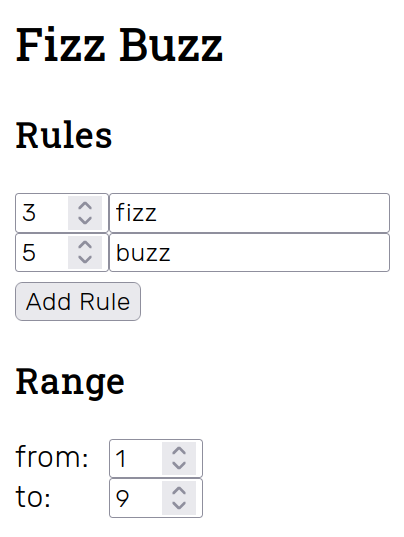
\includegraphics[width=.6\linewidth]{./mainmatter/pictures/fizzbuzz_control.png}
\captionof{figure}{Fizz Buzz controls} \label{fig:fizzbuzz_control}
\end{minipage}%
\begin{minipage}{.5\textwidth}
  \centering
  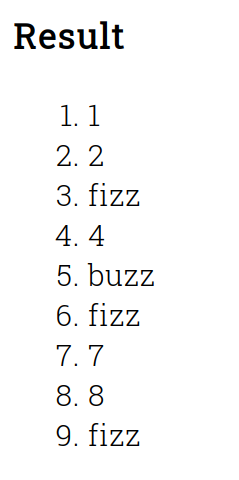
\includegraphics[width=.4\linewidth]{./mainmatter/pictures/fizzbuzz_result.png}
  \captionof{figure}{Fizz Buzz result}
  \label{fig:fizzbuzz_result}
\end{minipage}
\end{figure}

\subsection{JINQ}
\label{sub:results JINQ}
The following examples use |JINQ| to browse and process JSON files.

\subsubsection{Find all Students}
\label{subsub:Find all Students}
We want to filter out all participants that have a student ID. As you can see
in the excerpt of the JSON file in listing~\ref{lst:json_file_devs}, the
property |switch-edu-id| is not defined for all people. Because the
|JsonMonad| works in the background with a maybe, such situations can be
processed without null handling.

\begin{lstlisting}[
  style=json, 
  caption=Excerpt of a JSON File including developers,
  label={lst:json_file_devs}
  ]
[
  {
    "id": 1,
    "name": "",
    "age": 28,
    "salary": 50000,
    "favoriteLanguages": [1, 3, 5]
  },
  {
    "id": 2,
    "switch-edu-id": "12-432-23",
    "name": "Emma Johnson",
    "age": null,
    "salary": 60000,
    "favoriteLanguages": [2, 4]
  },
  {
    "id": 3,
    "name": "Sophia Davis",
    "age": 40,
    "salary": null,
    "favoriteLanguages": [null, 4, 5]
  },
  ...
 ]
\end{lstlisting}

Using JINQ it is straightforward to access the desired students by just using
the function |where|:

\begin{lstlisting}[
  style=ES6, 
  caption=JINQ Example - find all students,
  label={lst:jinq_find_students}
  ]
const findAllStudentIds = developers => {
  const allIds =
    from(JsonMonad(developers))
      .select(x => x['switch-edu-id'])
      .result();
};
\end{lstlisting}

\subsubsection{Find Sophia's Programming Languages}
\label{subsub:Find Sophia's Programming Languages}

This example combines two JSON files. We use the JSON file from the previous
example and the one from listing~\ref{lst:json_file_lang} below.
Listing~\ref{lst:jinq_sophias_langs} shows the code that finds Sophia's 
favourite programming languages by combining two JSON files using |pairWith|. 

\begin{lstlisting}[
  style=json, 
  caption=Excerpt of a JSON File including programming languages,
  label={lst:json_file_lang}
  ]
[
  {
    "id": 1,
    "name": "Java"
  },
  ...
  {
    "id": 4,
    "name": "C++"
  },
  {
    "id": 5,
    "name": "Haskell"
  }
]
\end{lstlisting}
This is also comparatively easy to do with JINQ. |pairWith| allows adding a
second data source to the current one, forming all possible combinations. The
function |where| then keeps only the needed pairs. A simple mapping at the end
outputs the names of the programming languages.
\begin{lstlisting}[
  style=ES6, 
  caption=JINQ example - find Sophia's programming languages,
  label={lst:jinq_sophias_langs}
  ]
const sophiasProgrammingLanguages = (devs, languages) =>
    from(JsonMonad(devs))
      .where   ( dev    => dev.name === "Sophia Davis")
      .select  ( sophia => sophia.favoriteLanguages)
      .pairWith( JsonMonad(languages) )
      .where   ( ([langId, language]) => langId === language.id )
      .select  ( ([     _, language]) => language.name )
      .result  ();
\end{lstlisting}

\subsection{Numerical Differentiation}
\label{sub:Numerical Differentiation}
This example shows a mathematical use case, the numerical differentiation using
sequences:

\begin{lstlisting}[
  style=ES6, 
  caption=Differentiation using sequences,
  label={lst:diff_sequences}
  ]
const halve   = x => x / 2;
const repeatF = (f, x) => _.Sequence(x, _ => true, f);
const halves = h0 => repeatF( halve, h0);

const slope = f => x => h => (f(x + h) - f(x)) / h;
const differentiate = h0 => f => x => _.map ( slope(f)(x) ) (halves(h0));
\end{lstlisting}

Listing~\ref{lst:diff_sequences} implements the following steps: 


\begin{itemize}
  \item{|repeatF| repeatedly applies the function $f$ to a value of the
    previous calculated result, starting with $x$.}
  \item{ |halves| is using |repeatF| and |halve| to halve a value $h0$.} 
    \item{|slope| calculates the slope of a function $f$ at the position $x$
      with delta $h$.}
 \end{itemize}

This code already provides everything needed for differentiation. The function
|differentiate| calculates the slope of a function at a given point $x$ more
and more exactly.
Listing~\ref{lst:diff_seq_parabola} uses these functions to determine the 
slope at $x = 1$ of the function |parabola| defined on line~\ref{line:diffs}:

\begin{lstlisting}[
  style=ES6, 
  caption=Differentiation using sequences,
  label={lst:diff_seq_parabola}
  ]
const parabola = x => x * x; *'\label{line:diffs}'*

const diffs = differentiate(0.5)(parabola)(1);
\end{lstlisting}

Since |diffs| contains an infinite sequence, one further
function is still needed.
Listing~\ref{lst:impl_within} shows the function |within|, which allows
differentiating until two successive values are smaller than a given epsilon:

\begin{lstlisting}[
  style=ES6, 
  caption=Implementation of within,
  label={lst:impl_within}
  ]
const within = eps => sequence => {
  const [a, rest] = _.uncons(sequence);
  const [b]       = _.uncons(rest);
  const diff      = Math.abs(a - b);

  if (diff <= eps) return b;
  return within(eps)(rest);
};
const slopeOfFAtX = within(0.000_1)(diffs);
\end{lstlisting}

Listing~\ref{lst:impl_within} defines the following implementations:

\begin{itemize}
  \item |within| calculates recursively the slope of the |parabola| using the
    sequence |diffs| until a satisfying accuracy. Because of the laziness of
    the sequence, |within| only calculates as many slopes as needed!
  \item At the end, |slopeOfFAtX| calculates the slope with the given parameters.
\end{itemize}


\subsection{Tic Tac Toe with a Kind of AI}
\label{sub:Alpha - Beta Algorithm}
This section describes the implementation of the alpha-beta heuristic in
JavaScript, an algorithm for estimating how good a position a game player is
in. \\ 
This algorithm allows for building a computer-controlled opponent for a
turn-based game. Hughes explains how the algorithm uses laziness and
higher-order functions to be modular and extensible in his paper.~\cite[p.
16]{hughes_why_1989}. As chapter~\ref{chap:Modularizing Programs} describes, the
Sequence library supports these two concepts, thus allowing to port the
algorithm to JavaScript.

\subsubsection{How does the Algorithm work?} % (fold)
\label{subsub:How does the Algorithm work?}
The following explanation is meant to give a brief overview for the
algorithm, allowing to understand the preceding code. For a deeper
understanding of the algorithm, consider ~\cite[Ch. 5]{hughes_why_1989} or the
section "Incremental Development" in Frege Goodness~\cite{frege_goodness}.

\paragraph{Building a Game Tree} The idea of the algorithm is to build a tree
containing \textit{all} possible playing fields. The start node in this
tree is the current state of the playing field. Its children are all possible
playing fields, which can arise when the players make their next moves. This
results in a potentially endless tree. All direct successors of a node are the
next possible moves for this node's playing field. Since this tree can be huge,
depending on the game, even infinitely large, only a lazy data structure can
handle it!\\
The algorithm must estimate whether a playfield is good or bad for a player to
find the best possible next move. The simplest way to figure this out is to
look at the playing field and decide if a player has already won. In the case
of tic tac toe, a player has won when three of his symbols are next to each
other. \\
A function (called |evalFunction|) does this evaluation - if the algorithm has
won the game on a field, it evaluates to 1 if it has lost to -1, in all other
cases, to 0.\\
The |evalFunction| is mapped over the tree (where higher-order functions come
into play) - each node is assigned its static value, saying how promising the
playfield of this node is. This results in a new tree with the value of
|evalFunction| assigned to the nodes instead of all possible fields.\\

\paragraph{What is the best Move?}
The tree's root is the current playing field - the algorithm cannot know from
the root which moves are good and which are not. The previously mentioned
|evalFunction| will evaluate to 0 for most nodes directly after the root.
Therefore, the computer also calculates subsequent moves. The values of the
lowest calculated nodes are then propagated upwards to the root. 

The function |maximize| goes through to the lowest precalculated level. It
evaluates the board there: when it is the computer's turn, it selects the board with
the highest value assigned (safest chance of winning). If it is the opponent's
turn, it selects the smallest value (the algorithm thus assumes that the
opponent also selects the best possible move). This found value is assigned to
the parent node as a result - and chooses the best move on this level according
to the same scheme. Ultimately, the root has the value with the best possible
chances of winning!

\paragraph{How to evaluate the huge Tree?} The tree of possible moves and possible
result values can be huge. So the algorithm must have a way to limit the tree
to a fixed depth. The algorithm uses pruning - from a freely selectable depth,
it cuts the children off. 

\subsubsection{Implementation}
\label{subsub:alphabeta_implementation}
\paragraph{Basic Types and Helper functions} 
Listing~\ref{lst:tictactoe_types} shows the required types for the game
implementation. \\
A pair models the |Tree| (line~\ref{line:ttt_treetype}) - the first
value is the current node, and the second value is a sequence consisting of
further trees. The types |Player| and |Stone| exist only for writing more
expressive JSDoc.

\begin{lstlisting}[
  style=ES6, 
  caption=Tic tac toe types,
  label={lst:tictactoe_types}
  ]
/**
 * 
 * @template _T_
 * @typedef {SequenceType<Tree<_T_>>} TreeSequence
 */

/** *'\label{line:ttt_treetype}'*
 * @template _T_
 * @typedef { PairSelectorType<_T_, TreeSequence<_T_>> } Tree
 */


/**
 * @typedef { "Computer" | "Human" | "NoPlayer" } Player
 */

/**
 * @typedef { 1 | -1 | 0 } Stone
 */

/**
 * @typedef Board
 * @property { Player } whosTurn
 * @property { Iterable<Stone>} fields - A board has fields from 0 to 8.
 */
\end{lstlisting}

Listing~\ref{lst:tictactoe_players} includes the definition of the players and some
functions used in the game process. Since JavaScript does not support pattern
matching, the functions |opponent| and |stone| use a workaround - they store
the mappings in an object.

\begin{lstlisting}[
  style=ES6, 
  caption=The players and some helper functions,
  label={lst:tictactoe_players}
  ]
/** @type { Player } */
const Computer = "Computer";

/** @type { Player } */
const Human = "Human";

/** @type { Player } */
const NoPlayer = "NoPlayer";

/**
 * Returns the opponent of a given player.
 * @param { Player } player
 * @return Player
 */
const opponent = player => {
  const pairings = {
    "Computer" : Human,
    "Human"    : Computer,
    "NoPlayer" : NoPlayer,
  };
  return pairings[player];
};

/**
 * Returns the stone number of a given player.
 * @param { Player } player
 * @returns Stone
 */
const stone = player => {
  const pairings = {
    "Computer" :  1,
    "Human"    : -1,
    "NoPlayer" :  0,
  };
 return pairings[player];
};

/**
 * Transforms each board element using the given function f.
 * @template _T_, _U_
 * @type {
 *         (f: (Board) => _T_)
 *      => (tree: Tree<_U_>)
 *      => Tree<_T_>
 * }
 */
const treeMap = f => ([a, sub]) => Pair(f(a))(map(treeMap(f))(sub));
\end{lstlisting}

\paragraph{Building trees and processing the Game Board} 
Listing~\ref{lst:tictactoe_gametree} shows the functions for building a game
tree. |unfold| is a function that takes a value (for example, a board) and
creates new values of the same types of it (for example, all boards possibly
arising in one move).
\begin{lstlisting}[
  style=ES6, 
  caption=Tic tac toe game tree,
  label={lst:tictactoe_gametree}
  ]
/**
 * Generates recursively a game tree, which is potentially endless.
 * @template _T_
 * @type {
 *       (unfold: ((_T_) => Iterable<_T_>))
 *    => (a: _T_)
 *    => Tree<_T_>
 * }
 */
const buildTree = unfold => a => {
  const as = unfold(a);
  const children = map(buildTree(unfold))(as);
  return Pair(a)(children);
};

/**
 * Creates a game tree.
 * @param { Board } board
 * @returns Tree<Board>
 */
const gameTree = board => buildTree(moves)(board);
\end{lstlisting}

Listing~\ref{lst:tictactoe_move} includes the |moves| function. This function
calculates all possible moves for a player based on the current playing field.
If a player has already won, it returns an empty sequence.
\begin{lstlisting}[
  style=ES6, 
  caption=Tic tac toe move function,
  label={lst:tictactoe_move}
  ]
/**
 * Indexes each field using a {@link PairType}.
 * @param { Iterable<Stone> } fields
 * @return { SequenceType<PairType<Stone, Number>> }
 */
const indexFields = fields => zip(fields)(Range(1,9));

/**
 * Calculates possible moves for a given board.
 * @param { Board } board
 * @return SequenceType<Board>
 */
const moves = board => {
  if (hasWon(board)(Computer)) return /**@type {SequenceType<Board>} */nil;
  if (hasWon(board)(Human))    return /**@type {SequenceType<Board>} */nil;

  const otherPlayer   = opponent(board.whosTurn);
  const indexedFields = indexFields(board.fields);

  const blankIndices =
    from(indexedFields)
      .where( ([content, _]) => content === stone(NoPlayer))
      .select( ([_, i]) => i)
      .result();

  const fieldsWithPlayerPlacedAt = pos =>
    from(indexedFields)
      .select(([content, i]) => i === pos ? stone(board.whosTurn) : content)
      .result();

  const boardFieldsAfterMove = map (fieldsWithPlayerPlacedAt) (blankIndices);

  return map(fields => ({fields, whosTurn: otherPlayer})) (boardFieldsAfterMove);
};
\end{lstlisting}

\paragraph{Evaluating a Board}
Listing~\ref{lst:tictactoe_hasWon} shows the implementation of the |hasWon|
function, which checks if a player has won on a given board. The evaluation
function, explained in section ~\ref{subsub:How does the Algorithm work?}, uses
this function to assess a playing field. Line~\ref{line:ttt_static_eval}
defines this function called |staticEval|.

\begin{lstlisting}[
  style=ES6, 
  caption=Tic tac toe hasWon function,
  label={lst:tictactoe_hasWon}
  ]
/**
 * Checks, if a player has won.
 * @type {
 *    (board: Board)
 *    => (player: Player)
 *    => Boolean
 * }
 */
const hasWon = board => player => {
  const winTriples = [
    [1,2,3], [4,5,6], [7,8,9], // row
    [1,4,7], [2,5,8], [3,6,9], // col
    [1,5,9], [3,5,7]           // diag
  ];

  const checkTriple = triple => {
    const actualStone   = stone(player);
    const indexedFields = indexFields(board.fields);

    const playerOnFields =
      from(indexedFields)
      .where( ([_, i])        => triple.includes(i))
      .select( ([content, _]) => content === actualStone)
      .result();

    return foldl$((acc, cur) => acc && cur, true)(playerOnFields);
  };
  return pipe(
    map(checkTriple),
    foldl$((acc, cur) => acc || cur, false)
  )(winTriples)
};

/**
 * Evaluates a given board.
 * @param { Board } board
 * @returns Number
 */
const staticEval = board => {*'\label{line:ttt_static_eval}'*
  if (hasWon (board) (Computer)) return 1.0;
  if (hasWon (board) (Human))    return -1.0;
  return 0.0;
};

\end{lstlisting}

\paragraph{Finding the best Move}
Listing~\ref{lst:tictactoe_minimax} shows the implementation of the functions
|maximize| (and its counterpart |minimize|) explained in
section~\ref{subsub:How does the Algorithm work?}. These functions determine
which are the best moves.

\begin{lstlisting}[
  style=ES6, 
  caption=Tic tac toe minimax algorithmus,
  label={lst:tictactoe_minimax}
  ]
/**
 * Determines the best move.
 * @template _T_
 * @param { Tree<_T_>}
 * @return { _T_ }
 */
const maximize = ([a, sub]) => {
  if (sub ["=="] (nil)) return a;
  return max$ (map(minimize)(sub))
};

/**
 * Determines the best move for the opponent.
 * @template _T_
 * @param { Tree<_T_>}
 * @return { _T_ }
 */
const minimize = ([a, sub]) => {
  if (sub ["=="] (nil)) return a;
  return min$ (map(maximize)(sub))
};
\end{lstlisting}

\paragraph{Pruning Trees} 
We cut off (prune) the possibly infinite tree. The following
listing~\ref{lst:tictactoe_prune} shows the implementation of this pruning.
Since subtrees are sequences, |nil| replaces them when pruning.

\begin{lstlisting}[
  style=ES6, 
  caption=Tic tac toe prune function,
  label={lst:tictactoe_prune}
  ]
/**
 * Prunes a given {@link Tree} to a max depth n.
 * @template _T_
 * @type {
 *           (n: Number)
 *        => (tree: Tree<_T_>)
 *        => Tree<_T_>
 * }
 * @param n
 */
const prune = n => tree => {
  const [a, sub] = tree;
  if (n === 0) return Pair(a)(nil);
  else return Pair(a)(map(prune(n-1))(sub));
};
\end{lstlisting}

\paragraph{Putting it all together}
The following functions evaluate a playing field. \\ 
The function |nextBoard| calculates the best possible next move for the
computer. The number |lookaheads| defines how many turns the algorithm
calculates in advance. Based on these calculations the algorithm chooses the
next move.

\begin{lstlisting}[
  style=ES6, 
  caption=Tic tac toe - evaluating functions,
  label={lst:tictactoe_eval}
  ]
/**
 * Evaluates a given Board by building a tree
 * @type {
 *            (lookahead: Number)
 *         => (board: Board)
 *         => Number
 * }
 */
const evaluate = lookahead => board => {
  const prunedTree = prune(lookahead)(gameTree(board));
  const mappedTree = treeMap(staticEval)(prunedTree);
  return minimize(mappedTree);
};

/**
 * @template _T_
 * @type {
 *            (lookahead: Number)
 *         => (board: Board)
 *         => PairSelectorType<_T_, Board>
 * }
 */
const nowValue = lookahead => board =>
  Pair(evaluate(lookahead)(board))(board);

/**
 * Calculates the next board with given board fields.
 * @type {
 *          (lookahead: Number)
 *       => (inFields: Array<Number>)
 *       => Board
 * }
 */
const nextBoard = lookahead => inFields => {
  const currentBoard = { whosTurn: Computer, fields: inFields };
  // get all possible
  const possibleMoves  = moves (currentBoard);
  if (isEmpty(possibleMoves)) return currentBoard;
  // evaluate each move by looking ahead how good it is
  let evaluatedMoves =  map (nowValue(lookahead)) (possibleMoves);

  // if the computer is sure to lose 
  // only look one place ahead to prevent the "nearest" loss
  if (onlyLoses(evaluatedMoves)) {
    evaluatedMoves = map (nowValue(1)) (possibleMoves);
  }

  /**
   * Gets the highest ranked board of the passed board
   * @param {SequenceType<PairSelectorType<Number, Board>>} boards
   * @return Board
   */
  return bestOf(evaluatedMoves);
};
\end{lstlisting}

\subsubsection{The Result} % (fold)
\label{sec:ttt_result}
One advantage of JavaScript is that it works hand in hand with websites and
HTML. A website with a UI (like figure~\ref{img:ttt_playfield}) can now use the
algorithm:\\

\begin{figure}[H]
    \centering
    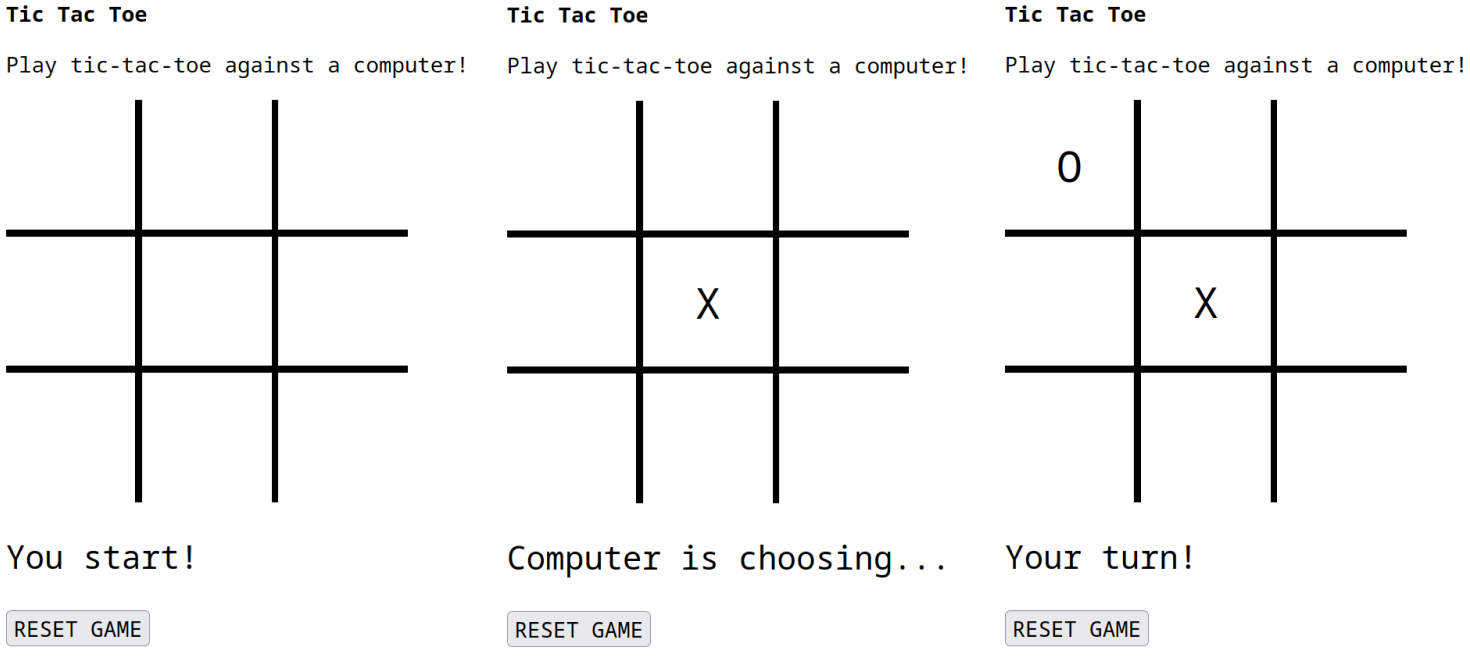
\includegraphics[width=0.9\textwidth]{./mainmatter/pictures/tic-tac-toe-field.png}
    \caption{A website using the algorithm}
    \label{img:ttt_playfield}
\end{figure}

When a player places his stone on the board, the function |nextBoard| gets
called. The algorithm automatically makes the best possible next turn based on
how many moves it can look ahead and returns the new board.
% subsubsection The result (end)

\subsubsection{Conclusion} % (fold)
\label{subsub:ttt_conclusion}
This example shows impressively how the Sequence library enables developers to
adapt an algorithm developed for functional programming languages in
JavaScript.\\
Of course, copying the algorithm is impossible because JavaScript misses some
language features like pattern matching. Nevertheless, the essential concepts
and logic of the algorithm can be adopted directly! \\
It is also exciting how JSDoc allows constructing straightforward talking types
like |Player| or |Stone| (listing~\ref{lst:tictactoe_types}).\\
To extend the algorithm, for example, to improve the static evaluation to
decide how good a current playing field is, only one function has to be
adjusted. Also, the evaluation of the algorithm can be easily improved and
detached from other logic by increasing the number of lookahead moves. Further
optimizations to prune away subtrees that are out of consideration anyway can
be done directly in the function |maximize|.\\
Thus, the modularity and extensibility of the program is very high.
% subsubsection Conclusion (end)

\section{Future Features}
\label{sec:Future Features}
This chapter covers unimplemented functions. These include implementations that
were no longer possible during the work or resulted from user testing feedback.
The following articles describe the most relevant features and explain why it
makes sense to implement them at a future point in time.

\subsection{Logging}
\label{sub:Logging}
Logging is a topic that has come up several times. It appears, on one hand,
during the implementation of the Sequence Library, but also through as feedback
from a test proband. In our computer science project work from the fifth
semester IP5 we had to implement a logging framework. This would also be useful
to include in the Sequence Library. Especially in case of errors, analyzing
messages from the involved functions would be helpful. Currently, the logging
framework is only included in a part of the test framework. But this could be
extended in a next step.

\subsection{Operators and Operations}
\label{sub:Operators and Operations}

\subsubsection{uncons}
\label{subsub:uncons}
|uncons| is an operation that returns the first and the rest of an iterable in a
pair. Basically, this operation is already included in the sequence library.
But only as an un-safe variant. That means, |uncons| applied to an empty list
fails. Thus one would have a version, which for example, wraps the result in a
|MaybeType|. |uncons| on an empty list would then return |Nothing|. The
api documentation page~\cite{hoogle_uncons} describes the function in detail.

\subsubsection{tail}
\label{subsub:tail}
|tail| ~\cite{hoogle_tail} is a useful function that removes the first element of an |Iterable|
and returns the rest of it. By implementing tail, one have to pay attention to
empty |Iterable| single element case. An option could be to return a
|MaybeType|. |Nothing|, if the list has one or zero elements, and
|Just| including the result otherwise.

\subsubsection{unfoldr}
\label{subsub:unfoldr}
|unfoldr| is a powerful concept of creating sequences of data. It would
supplement the options to make new |Iterable| beside the |Sequence|
constructor. It works on a |MaybeType|. |unfoldr| creates an |Iterable| which returns
a |PairType| wrapped in Just with the value of the current iteration and the next
element. If the stop condition is fulfilled, |unfoldr| return |Nothing|. For
further information, have a look at the documentation on hoogle~\cite{hoogle_unfoldr}.

\subsubsection{iterate}
\label{subsub:iterate}
|iterate| takes two arguments. The first argument is a function, and the second
is a start value. It generates an infinite |Iterable| of repeated applications of
the function to the calculated value. You will find more information about
|iterate| on hoogle~\cite{hoogle_iterate}.

\subsection{JINQ Functions}
\label{sub:JINQ Functions}
It is possible to get errors when working with JINQ and JSON Monad by grabbing
not present values. That means if a function in select accesses a property
which is not defined, it will throw an error. This kind of null-case handling
takes a lot of work. To remedy this situation, having error-safe functions like
|safeSelect| to access probably present values would be excellent.

\subsection{Applications}
\label{sub:Applications}
\subsubsection{Fixpoint Sequence}
\label{subsub:Fixpoint Sequence}
In the mathematical context, having a tool for approximations is helpful. A
constructor for such a case could be the Fixpoint Sequence. It allows us to
find an approximation with a given number of iterations or by providing a value
of minimal deviation.

\subsubsection{A Kind of Scalpel}
\label{subsub:A Kind of Scalpel}
Scalpel~\cite{scalpel} is a Haskell library to scrap web content. Building a similar
application based on the present implementations could be possible. With JINQ
and |JsonMonad|, we already have a scraping tool for JSON Objects. A future
implementation could use a similar approach to develop such an application.

\section{Conclusion}
\label{sec:conclusion}
This Chapter discusses the results and findings of the thesis. The beginning reflects the
standard library we created in this thesis and its achievements. The following
Sections deal with more topic specific aspects. Therefore, we make a
recap of particular decisions during development. Finally, non-functional
aspects are in the foreground, where we see what other values were important to
us while implementing the project.

\subsection{Findings and Achievements}
\label{sub:Findings and Achievements}
The objective of this thesis was to develop a functional standard library for
the Kolibri Web Ui Toolkit in JavaScript. To achieve this, we delved into the
iterable protocols of JavaScript, leveraging our understanding to construct the
concept of Sequences. Sequences are characterized by their lazy evaluation and
immutability, offering a powerful tool for handling any iterable object. By
employing the decorator approach, we built various functionalities capable of
processing regular JavaScript arrays and other iterables. This was made
possible by passing the receiver to the function, which also allows us to take
advantage of eta reduction.
\newline
An excellent example of this is the pipe function, enabling the execution of
multiple operations in a sequential manner, similar to what can be achieved
with Java Streams. With the Sequence Library's compatibility with all iterable
objects, it became logical to make other existing collections iterable as well.
As a result, we extended the Kolibri Toolkit's existing collections such as
Pair, Stack, and Tuple to support iterability. Additionally, we implemented
specialized Sequences that facilitate the generation of application-specific
data, such as the |AngleSequence|, which produces angles at regular intervals,
or a Sequence of prime numbers.
\newline
To ensure clarity and maintain consistency, all implementations are typed using
jsDoc. While overall the process went smoothly, we encountered limitations when
combining multiple types, as outlined in the thesis. Despite these challenges,
we made significant progress in developing a functional standard library for
the Kolibri Web Ui Toolkit, offering enhanced functionality and versatility to
JavaScript developers.

\subsection{A Closer Look to Particular Findings}
\label{sub:A Closer Look to Particular Findings}

\subsubsection{Similarity to Haskell}
\label{subsub:Similarity to Haskell}
As Haskell is a well-established and widely used functional language, we
frequently draw inspiration from its problem-solving approaches when making
decisions. In each case, this has proven to be a valuable choice. However, it
is essential to note that certain remarkable language concepts from Haskell
could not be directly adopted in JavaScript. Nevertheless, specific
implementations are pretty similar, as the following Listings~\ref{lst:comparing_with_javascript} 
and~\ref{lst:comparing_with_haskell} demonstrates.

\begin{lstlisting}[
  style=Haskell, 
  caption=Haskell vs. Sequence library - Haskell implementation, 
  label={lst:comparing_with_javascript}
  ]
-- Creating a list from 0 to 4
let list = unfoldr (\x -> if x < 5 then Just(x, x + 1) else Nothing) 0

-- mapping the list
map (\x -> x * 2) list 
\end{lstlisting}

\begin{lstlisting}[
  style=ES6, 
  caption=Haskell vs. Sequence library - JavaScript implementation,
  label={lst:comparing_with_haskell}
  ]
// Creating a list from 0 to 4
const list = Sequence(0, x => x < 5, x => x + 1);

// mapping the list
map(x => x * 2)(list)
\end{lstlisting}


\subsubsection{Robust Programming in JavaScript}
\label{subsub:Robust Programming in JavaScript}
Strange situations arise in JavaScript more often than in other programming
languages. One contributing factor is the nature of its type system. However,
within this thesis, we have demonstrated that it is still possible to program
reasonably robustly by leveraging functional programming concepts. Crucially,
this requires taking advantage of the functional aspects inherent to the
language, such as higher-order functions and partial application. Nonetheless,
we encountered certain limitations along the way. In particular, not all
desired behaviors can be achieved when dealing with the type system.
An illustrative example is the combination of a |MonadType| with an |Iterable|
type. When a function returns a  |MonadType|, the valuable information that could
have been preserved as Iterable is lost. Resolving such a situation requires
type-casting.

\subsubsection{Monadic Structures}
\label{subsub:Monadic Structures}
With |JINQ|~\ref{sec:Query different Data Structures}, we have realized an
concept based on monadic types. Thus, we could show that it is also
possible and valuable to implement such concepts in JavasScript.
This opens numerous possibilities for extensions that act on monadic types in
JavaScript.

\subsubsection{Testing}
\label{subsub:Testing}
A key ingredient for achieving a robust and sustainable library lies in having
a reliable test framework. In the case of the Sequence library, stability was
attained through the utilization of the TestingTable and configured Test
Objects~\ref{sec:Testing}, which provided a solid foundation for incremental growth.
By gradually incorporating new functionalities and corresponding test cases,
the core of the library became increasingly robust. Moreover, novel test
concepts were introduced during the development process to enhance the testing
capabilities further. A notable example is the introduction of invariant tests~\ref{subsub:Invariant Testing},
which systematically assess the behaviors of functionalities through
diverse testing approaches, ensuring comprehensive validation.

\subsection{Non-Functional Findings}
\label{sub:Non-Functional Aspects}

\subsubsection{Library Organization}
\label{subsub:Library Organisation}
During the development of the Sequence library, we consistently paid close
attention to non-functional aspects. As part of this effort, we adjusted the
organization of the project's development setup. This led us to the current
state, where each functionality is located in its own separate file. The
adoption of such a project structure has had a significant impact on the
overall clarity and navigability of the codebase. Moreover, it contributes to a
sense of order, which, in turn, enhances the overall code quality.
Additionally, it helps to prevent cycling dependencies when importing
particular functionalities.

\subsubsection{Code Quality}
\label{subsub:Code Quality}
By maintaining high code quality standards, we created a clear and consistent
code base. We paid attention to the following points:

\begin{itemize}
  \item{No code duplications}
  \item{Good naming}
  \item{Standardized formatting}
  \item{Only necessary exports of functions}
  \item{Appropriate comments}
  \item{Project organization and structure}
\end{itemize}

Strict adherence to these principles makes development easier for us and helps
library users find their way around more quickly. Additionally, it facilitates
future developers to learn how to add new functionalities.

\subsection{User Testing}
\label{sub:User Testing}
The user testing conducted in Section~\ref{sub:User Testing} was crucial for further improvement
of the Sequence library. It provided us with valuable feedback from programmers
who had no prior knowledge of the library. This insight allowed us to address
specific issues promptly and immediately improve based on the test results.
Additionally, we added other valuable suggestions to the list of potential
enhancements, as outlined in Chapter~\ref{sec:Future Features}.

